% !TEX root = ./main.tex
% ========================================================================== %
\section{Validation on simulations} \label{sec:simu}

In order to ensure that \panco\ is able to recover accurate pressure profile measurements, we test it on simulated inputs.
In this section, we detail this validation process, from the creation of the dataset to the results produces by \panco.
For reproducibility purposes, the datasets created and used for this analysis are made public with the software.

% -------------------------------------------------------------------------- %
\subsection{Sample selection}

The goal of the validation is to ensure that \panco\ is able to recover accurate pressure profiles from different types of data.
To that end, we seek to create realistic synthetic cluster maps from three instruments: the \textit{Planck} satellite, the South Pole Telescope (SPT), and the NIKA2 camera at the IRAM 30 m telescope.
The choice of these three instruments is motivated by their vastly different angular resolutions: the Compton$-y$ maps built from \textit{Planck} and SPT data have angular resolutions (expressed as the full width at half maximum, or FWHM) of 10 and 1.25 arcmin, respectively \citep{planck_collaboration_planck_2016, bleem_cmbksz_2022}, and the beam of the NIKA2 camera 150 GHz band -- used for tSZ mapping -- has an FWHM of 18 arcsec \citep{perotto_calibration_2020}.

We choose to create SZ maps for three clusters, labeled (C1, C2, C3), covering different regions of the mass-redshift plane:
\begin{alignat}{2}
    \nonumber {\rm C1}:\; & z=0.05,\ & M_{500} = 9 \times 10^{14} \ M_\odot ;\\
    \nonumber {\rm C2}:\; & z=0.5,\  & M_{500} = 6 \times 10^{14} \ M_\odot ;\\
              {\rm C3}:\; & z=1,\    & M_{500} = 3 \times 10^{14} \ M_\odot,
    \label{eq:valid:clusters}
\end{alignat}
These mock clusters are shown as black stars in figure~\ref{fig:valid:sample}.
The top panel shows their positions in the mass-redshift plane, indicating that C1, C2 and C3 are realistic detections for the \textit{Planck}, SPT, and ACT tSZ surveys, respectively.
Tbe bottom panel of figure~\ref{fig:valid:sample} places the clusters in the angular diameter-redshift plane, showing that C1 can be resolved in \textit{Planck}, SPT, and NIKA2 tSZ maps, while C2 and C3 are too small to be resolved by \textit{Planck}.

\begin{figure}[tp]
    \centering
    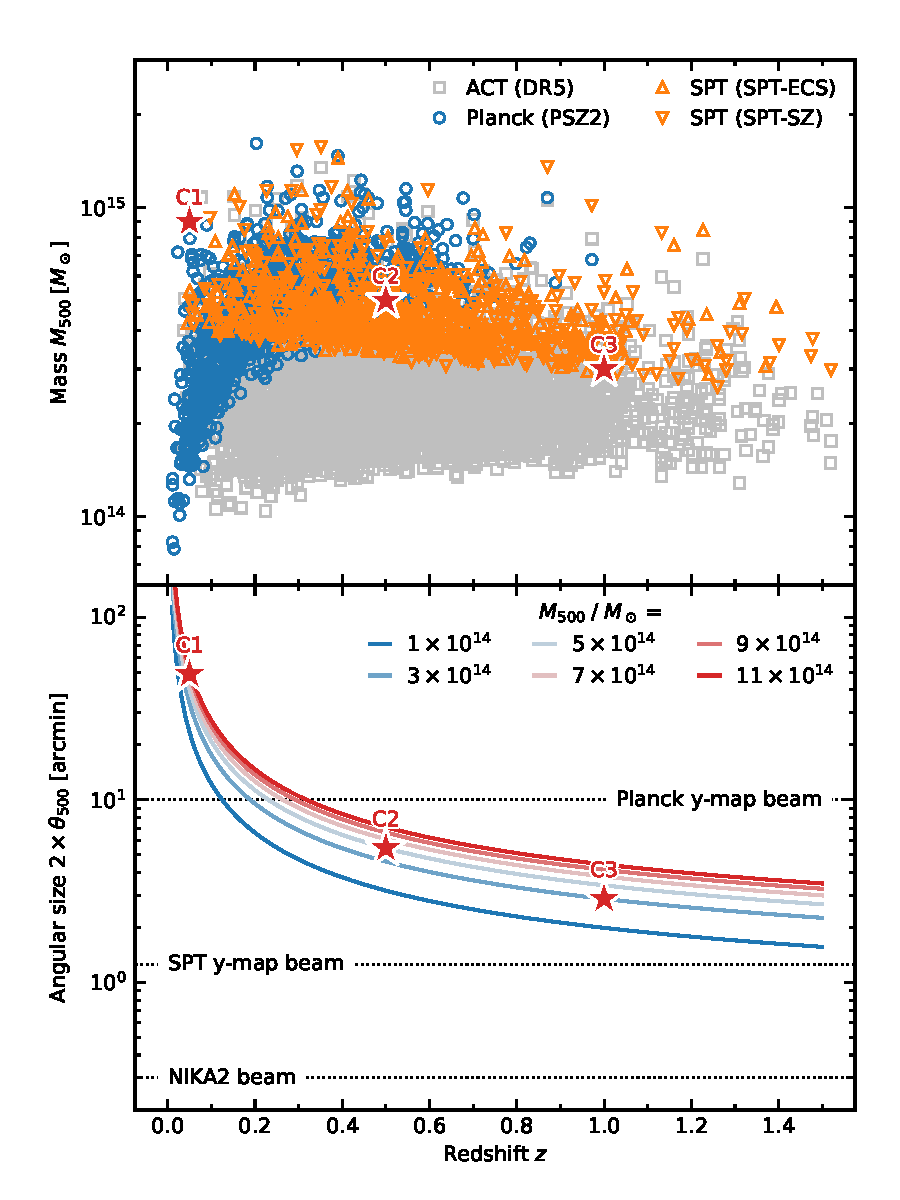
\includegraphics[width=\linewidth]{Figures/validation_sample.pdf}
    \caption{
        Validation cluster sample (black stars) in the mass-redshift plane (\textit{top panel}) and in the angular size-redshift plane (\textit{bottom panel}).
        For illustration, the top panel includes clusters detected in recent tSZ surveys: \textit{Planck} \citep{planck_collaboration_planck_2016-2}, ACT \citep{hilton_atacama_2021}, and SPT \citep{bleem_sptpol_2020,bleem_galaxy_2015}.
        Note that the redshift axis is truncated to $z<1.6$, therefore not showing all clusters in these samples.
        Colored lines in the bottom panel show the evolution of the angular $2\times\theta_{500}$ with redshift for clusters of different masses.
        The angular resolutions of the \textit{Planck} and SPT $y-$maps, as well as that of the NIKA2 camera at 150~GHz, are represented as dotted horizontal lines.
    }
    \label{fig:valid:sample}
\end{figure}

% -------------------------------------------------------------------------- %
\subsection{Data generation} \label{sec:simu:mkdata}

\begin{table*}[htp]
    \centering
    \begin{tabular}{l c c c c c}
        \toprule
        Instrument & Map size & Pixel size & FWHM & Filtering & White noise \\
        (Clusters) & $\theta_{\rm map}$ & $\theta_{\rm pix}$ & $\theta_{\rm FWHM}$ & & level \\
        \midrule
        \textit{Planck} & \multirow{2}{*}{$5\degree$} & \multirow{2}{*}{$2'$} & \multirow{2}{*}{$10'$} & \multirow{2}{*}{--} & Homogeneous \\
        (C1) & & & & & RMS=$4.12 \times 10^{-6} \; [y]$ \\
        \midrule
        SPT & \multirow{2}{*}{$1\degree$} & \multirow{2}{*}{$15''$} & \multirow{2}{*}{$1.25'$} & -- & Homogeneous, \\
        (C1, C2) & & & & & RMS=$9.78 \times 10^{-6} \; [y]$ \\
        \midrule
        NIKA2 & \multirow{2}{*}{$6.5'$} & \multirow{2}{*}{$3''$} & \multirow{2}{*}{$18''$} & NIKA2-like & Isotropic \\
        (C2, C3) & & & & transfer function & NIKA2-like RMS \\
        \bottomrule
    \end{tabular}
    \caption{\normalfont
        Properties of simulated maps emulating cutouts of the \textit{Planck} \citep{planck_collaboration_planck_2016} and SPT \citep{bleem_cmbksz_2022} $y-$maps, and NIKA2 cluster observations \citep{keruzore_exploiting_2020}.
    }
    \label{tab:simu:map_props}
\end{table*}


We create mock maps for the three clusters by forward modeling their tSZ signal.
We assume that each cluster has a pressure profile that follows the universal profile of \aten, scaled with its mass and redshift.
This pressure distribution is integrated along the line of sight to obtain a Compton$-y$ map.
This map is then projected on a flat-sky grid and convolved with a Gaussian filter to account for instrumental filtering, and added to a random noise realization.

As discussed previously, and illustrated in the bottom panel of figure~\ref{fig:valid:sample}, the angular size of each cluster is very different, and the mapping of their tSZ signal is very different for all instruments considered.
We therefore create different sets of maps for the three clusters.
For C1, the most extended cluster, we create mock \textit{Planck} and SPT maps.
For C2, our intermediate case, we create SPT and NIKA2 mock maps.
Finally, for C3, the smallest cluster in our sample, we only create mock NIKA2 data.
The characteristics of the maps are designed to mimic know cluster observations by the three instruments, and summarized in table~\ref{tab:simu:map_props}.
The generated maps are shown on the left panels of figure~\ref{fig:valid:dmr_2d}.

\paragraph{Planck-like data}  % ............................................ %
Our mock \textit{Planck} dataset is designed to emulate the \textit{Planck} Compton$-y$ map of \citet{planck_collaboration_planck_2016}.
The original data products for this map are in \texttt{healpix} format, which \panco\ cannot process, as it relies on the flat-sky approximation.
We therefore create maps of $(5\degree \times 5\degree)$ patches of the sky using a gnomonic projection, with a pixel size of $2'$, and a Gaussian PSF of ${\rm FWHM} = 10'$.
The noise in these maps is white and has an homogeneous distribution, with an RMS taken from the left panel of figure~13 in \citet{planck_collaboration_planck_2016}.
\todo{filtering?}
\todo{correlated noise?}

\paragraph{SPT-like data}  % ............................................... %
Our SPT-like maps mimic the plublicly available $y-$maps released by the SPT collaboration \citep{bleem_cmbksz_2022}.
We use the same projection as their flat-sky maps, \ie\ a Sanson-Flamsteed projection with $15''$ pixels, on a $(1\degree \times 1\degree)$ patch of the sky.
The resolution of the map is Gaussian with ${\rm FWHM} = 1.25'$.
We inject a white noise realization, the amplitude of which is evaluated by computing the RMS of the map in a $(5\degree \times 5\degree)$ patch of the sky, taking care of masking sources.
\todo{filtering?}
\todo{correlated noise?}

\paragraph{NIKA2-like data}  % ............................................. %
Our NIKA2-like data imitates the NIKA2 150~GHz sky maps obtained by the NIKA2 SZ Large Program \citep{mayet_cluster_2020, perotto_nika2_2021}.
In particular, we use the data products publicly released in \citet{keruzore_exploiting_2020}.
We create a gnomonic projection of a $(6.5' \times 6.5')$ patch of the sky with $3''$ pixels.
The angular resolution of the map is Gaussian with ${\rm FWHM} = 18''$, and we also take into account filtering of angular scales due to data processing via the transfer function of \citet{keruzore_exploiting_2020}.
The noise in these NIKA2 maps is considered white and isotropic, but not homogeneous, as the NIKA2 on-the-fly scanning strategy used for obsevations of the NIKA2 SZ Large Program creates a variation in the noise level of the maps depending on the distance from the pointing coordinates.
To accurately take into account this effect, we use the noise RMS map of \citet{keruzore_exploiting_2020}, which we multiply by a scalar value to account for different exposure times.
Data produced by the NIKA2 collaboration is in NIKA2 150 GHz surface brightness units, usually presented in mJy/beam.
The conversion coefficient of $y-$to$-$mJy/beam can be evaluated by integrating the tSZ spectral distortion in the NIKA2 150 GHz effective bandpass (accounting for atmospheric opacity at the time of the observations), and is usually of the order of $-12$ mJy/beam/$y$ \citep[\eg][]{keruzore_exploiting_2020}, therefore we choose this value for our map generation.

% \begin{figure*}[t]
%     \centering
%     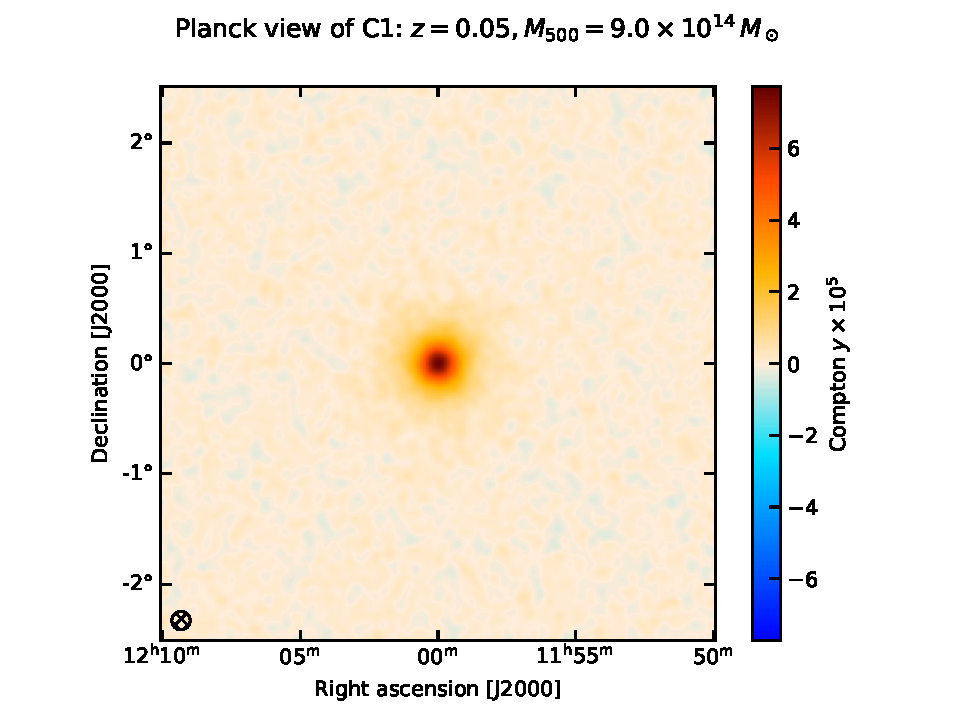
\includegraphics[page=1, width=0.49\linewidth, trim={1cm 0cm 1cm 1cm}, clip]{../validation/sim_maps.pdf}
%     \includegraphics[page=2, width=0.49\linewidth, trim={1cm 0cm 1cm 1cm}, clip]{../validation/sim_maps.pdf}
%     \includegraphics[page=3, width=0.49\linewidth, trim={1cm 0cm 1cm 1cm}, clip]{../validation/sim_maps.pdf}
%     \includegraphics[page=4, width=0.49\linewidth, trim={1cm 0cm 1cm 1cm}, clip]{../validation/sim_maps.pdf}
%     \includegraphics[page=5, width=0.49\linewidth, trim={1cm 0cm 1cm 1cm}, clip]{../validation/sim_maps.pdf}
%     \caption{%
%         Simulated maps of the three validation clusters.
%         \textbf{Top:} C1 seen by \textit{Planck} (\textit{left}) and SPT (\textit{right});
%         \textbf{Middle:} C2 seen by SPT (\textit{left}) and NIKA2 (\textit{right});
%         \textbf{Bottom:} C3 seen by NIKA2.
%         Map properties are summarized in table~\ref{tab:simu:map_props}, and the cluster properties in eq.~(\ref{eq:valid:clusters}).
%         Each map is smoothed with a Gaussian filter with $\sigma = 1 \; {\rm pixel}$ for displaying purposes.
%         The FWHM of the angular resolution of each map is shown as a hatched circle in its bottom left.
%     }
%     \label{fig:valid:maps}
% \end{figure*}

% -------------------------------------------------------------------------- %
\subsection{Pressure profile fitting}

The five generated maps are then used to extract a pressure profile using \panco, \ie\ following the procedure detained in \S\ref{sec:algo}.
We assume that we know the characteristics of the map prior to fitting -- \ie\ the width of the beams used, the transfer function, and the noise RMS given to \panco\ in input are the same ones that have beed used to generate the maps.

Two ingredients in our model then remain to be specified: the radial binning -- \ie\ the value of the radii $R_i$ in eq.(~\ref{eq:algo:pressure_profile}) -- and the priors on the parameters.
For the radial binning, we choose one that is identically determined by the angular coverage of each map.
The first bin is defined as the projected radius corresponding to the size of a map pixel, $R_0 = \mathcal{D}_{\rm A}(z) \tan^{-1} \theta_{\rm pix}$, where $\mathcal{D}_{\rm A}(z)$ is the angular diameter distance to the cluster redshift $z$.
Four bins $\left\{R_1 \dots R_4 \right\}$ are then added, log-spaced between the projected sizes of the beam FWHM, $\mathcal{D}_{\rm A}(z) \tan^{-1} \theta_{\rm FWHM}$, and of the half map size, $\mathcal{D}_{\rm A}(z) \tan^{-1} \theta_{\rm map} / 2$.

The priors on each parameter is defined as follows.
For the pressure parameters $P_i$, corresponding to the value of the pressure profile at radii $R_i$, we compute the value of the universal pressure profile from \aten\ for the cluster's mass and redshift.
The prior on $P_i$ is then set as a log-uniform distribution around this value:
\begin{equation}
    \label{eq:simu:prior_Pi}
    p(P_i) = \log\mathcal{U}(10^{-2}, 10^2) \times P_{\rm A10}(R_i).
\end{equation}
The prior on the conversion coefficient is set as a Gaussian distribution.
For \textit{Planck}- and SPT-like maps, the data is directly in units of Compton$-y$, therefore this distribution is centered around 1.
For NIKA2 data, as discussed in \S\ref{sec:simu:mkdata}, the central value of the prior is set at $-12$ mJy/beam/$y$.
For all data, the spread of the distribution is taken as $10\%$ of its central value.
Finally, the prior on the zero-level of the map is set as \todo{what did I put?}.

The MCMC sampling is run as presented in \S\ref{sec:algo:mcmc}, with $30$ walkers, and setting $n_{\rm auto} = ?$ and $\Delta\tau_{\rm max} = ?$ \todo{values?}.
For our tests, we used a 2021 MacBook Pro with an M1 Pro chip and a 10-core CPU \todo{is this necessary?}.
With this setup and these criteria, each fit took 10 to 20 minutes to converge.
The raw Markov chains are then saved, and cleaned for the exploitation as described in \S\ref{sec:algo:outputs}, with $n_{\rm burn} = ?$, $n_{\rm discard} = ?$, and $q_{\rm extr} = ?$ \todo{values}.

% -------------------------------------------------------------------------- %
\subsection{Results} \label{sec:simu:results}

The results of the regression is presented in Figures~\ref{fig:valid:dmr_2d} and \ref{fig:valid:profiles}.
Figure~\ref{fig:valid:dmr_2d} shows, for each of the five datasets, the simulated data (left), best-fitting 2D model (center), and the residuals (right).
The residuals panels show no significant structure, providing a visual indication of goodness of fit.
The right panels of Figure~\ref{fig:valid:profiles} also shows the data, model, and residuals, but as 1D azimuthal profiles, and include uncertainty computed from the spread of the sampled posterior.
The compatibility of the green curves (\ie\ residuals) with zero within uncertainties proves that \panco\ is able to retrieve a pressure profile that fits the data.

The left panels of Figure~\ref{fig:valid:profiles} show the pressure profiles recovered for each fit as the blue curves, including uncertainties.
The true profile used to generate each map data (\ie\ the universal \aten\ pressure profile for the cluster's mass and redshift, see \S\ref{sec:simu:mkdata}) is shown as a black dashed line.
For each data set, the agreement between the two curves across the considered radial range (\ie\ from the projected pixel size to the projected half map size) shows that \panco\ is able to retrieve an accurate estimation of the pressure profile of a cluster from its tSZ map.

\begin{figure*}[t]
    \centering
    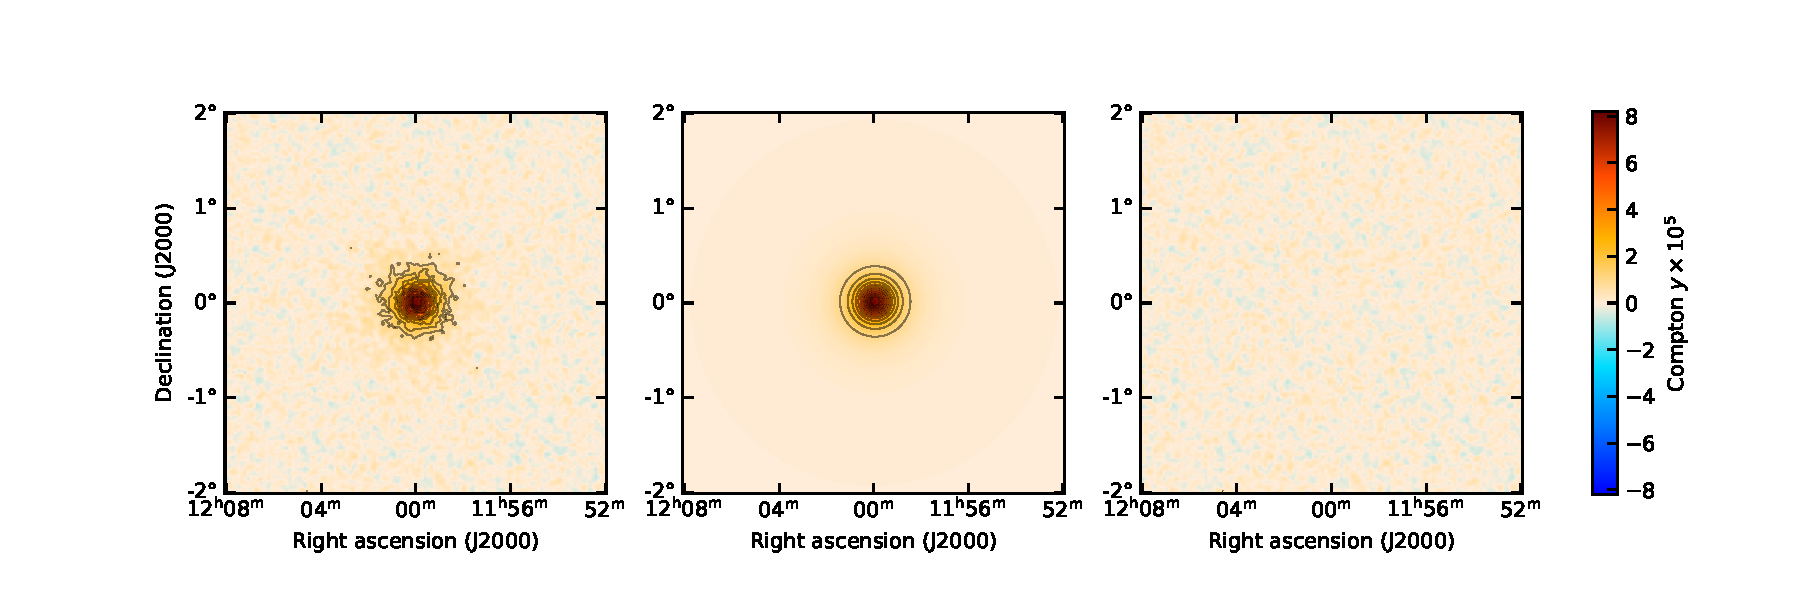
\includegraphics[height=4cm, trim={2cm 0.7cm 1.5cm 1.5cm}, clip]{../validation/results/C1/Planck/data_model_residuals_maps.pdf}
    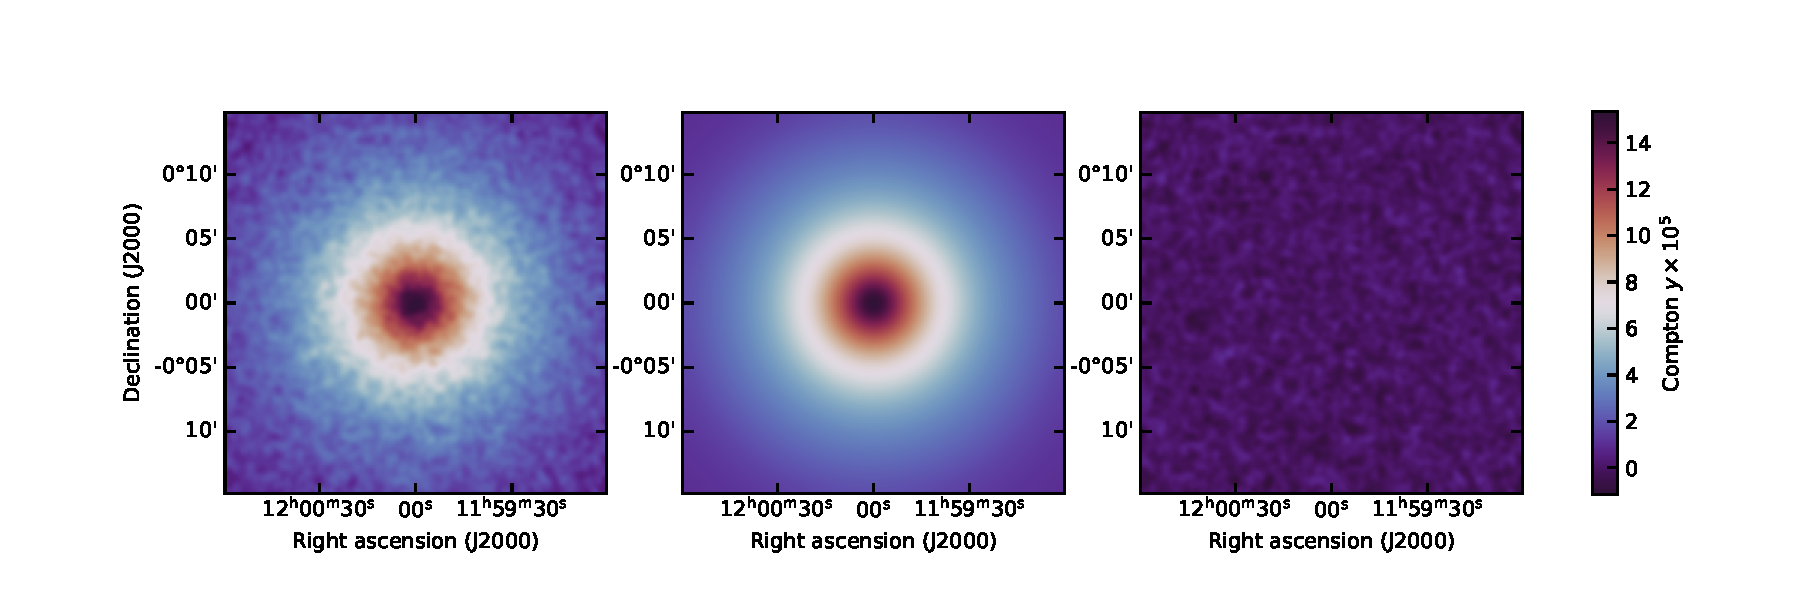
\includegraphics[height=4cm, trim={2cm 0.7cm 1.5cm 1.5cm}, clip]{../validation/results/C1/SPT/data_model_residuals_maps.pdf}
    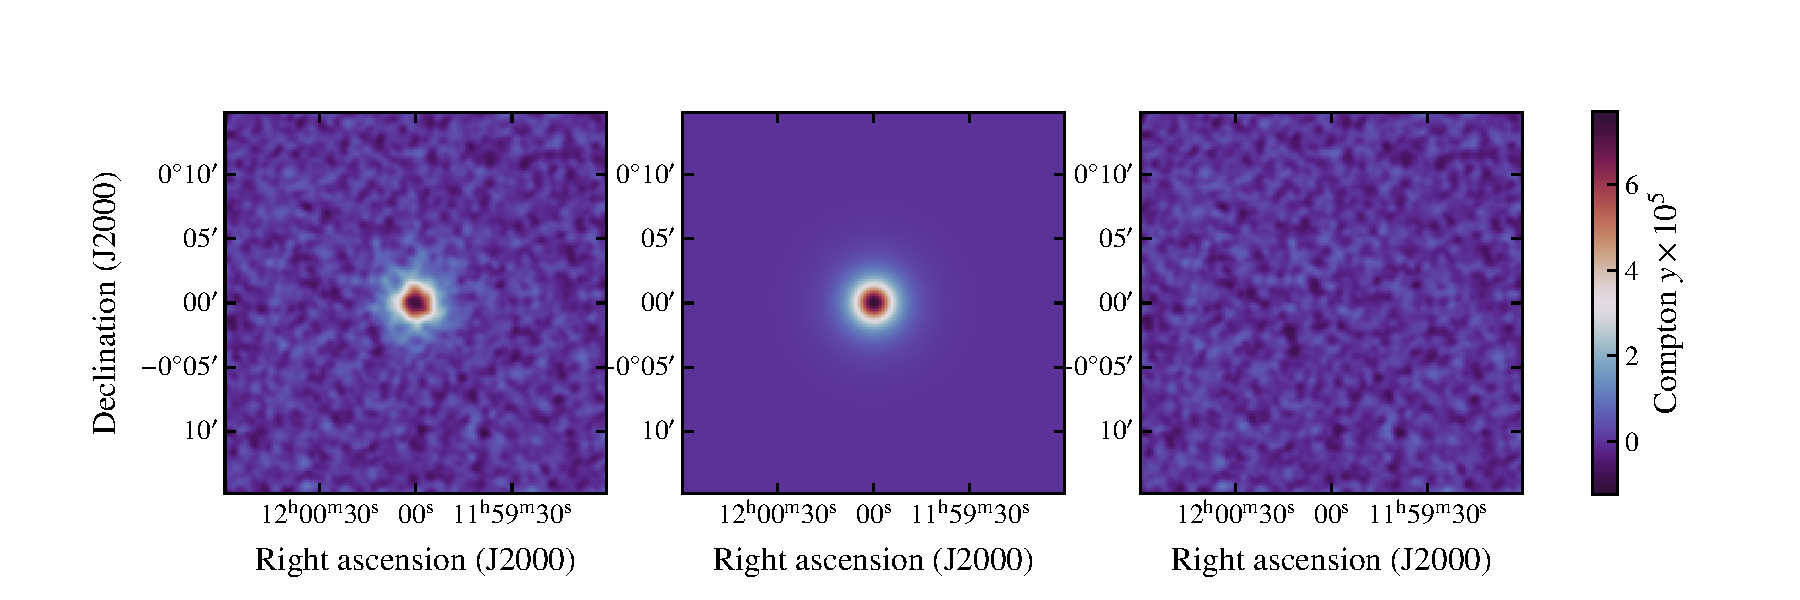
\includegraphics[height=4cm, trim={2cm 0.7cm 1.5cm 1.5cm}, clip]{../validation/results/C2/SPT/data_model_residuals_maps.pdf}
    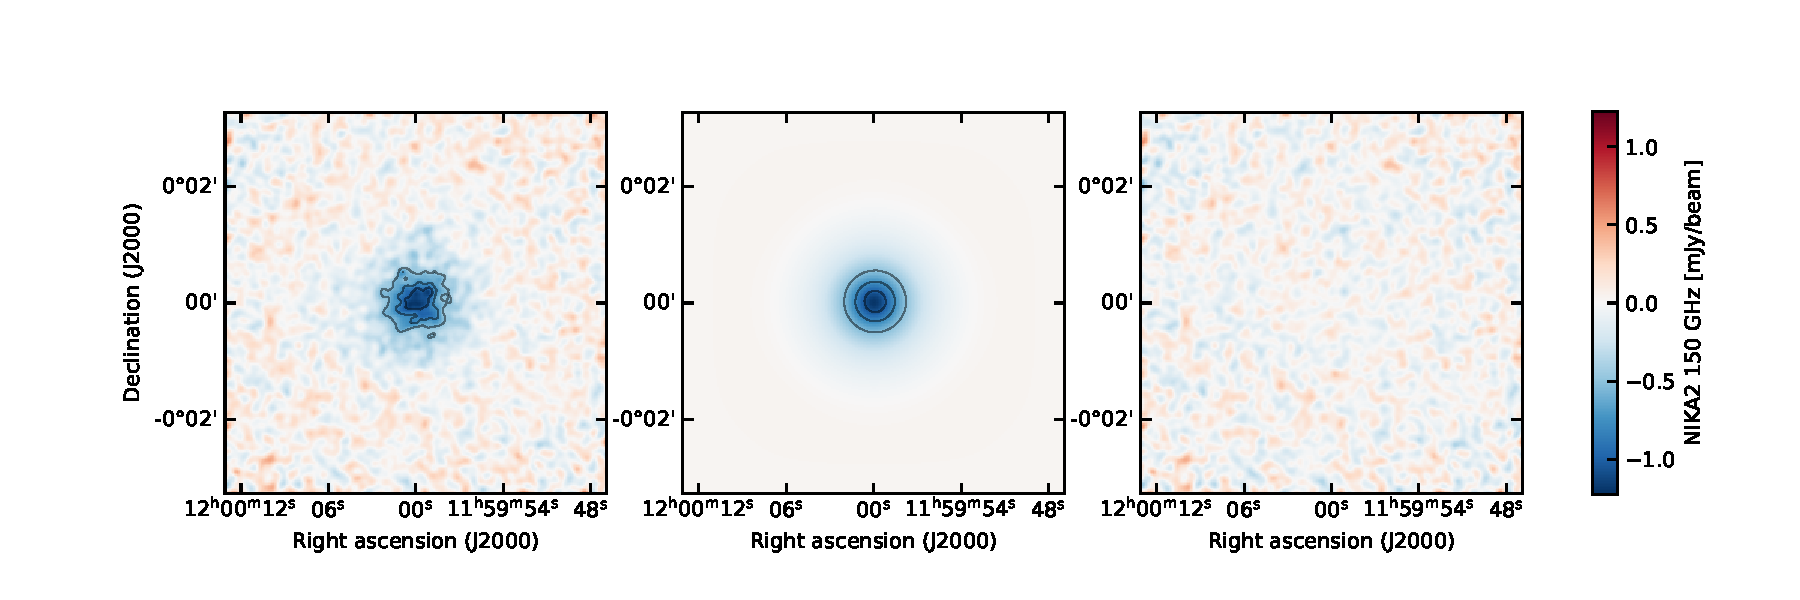
\includegraphics[height=4cm, trim={2cm 0.7cm 1.5cm 1.5cm}, clip]{../validation/results/C2/NIKA2/data_model_residuals_maps.pdf}
    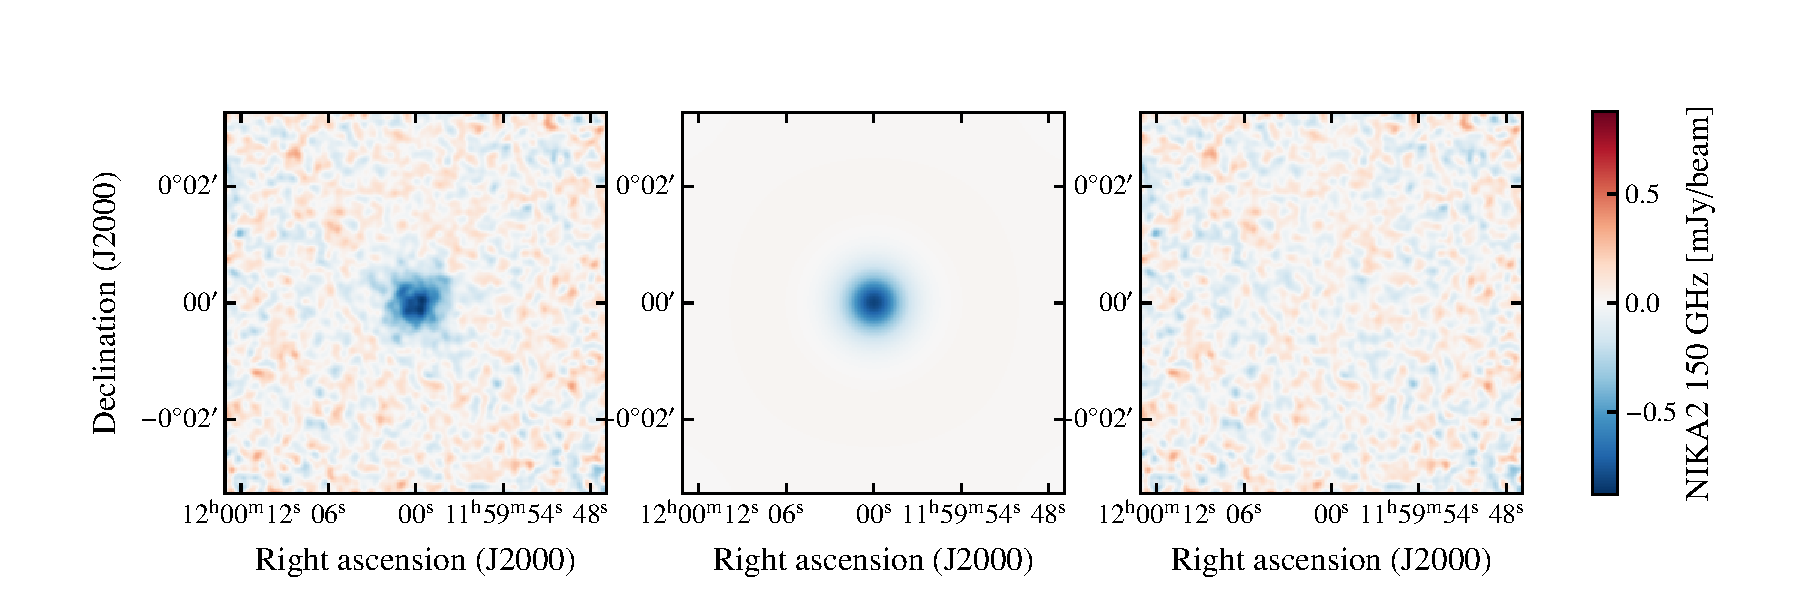
\includegraphics[height=4cm, trim={2cm 0.7cm 1.5cm 1.5cm}, clip]{../validation/results/C3/NIKA2/data_model_residuals_maps.pdf}
    \caption{
        Data (\textit{left}), model (\textit{center}), and residuals (\ie\ difference between data and model, \textit{right}) for the five validation fits:
        from top to bottom, C1 with \textit{Planck}, C1 with SPT, C2 with SPT, C2 with NIKA2, C3 with NIKA2.
        Maps are smoothed by a $1$ pixel Gaussian for display purposes.
        Grey curves are signal-to-noise isocontours, starting at $3\sigma$ with a $2\sigma$ spacing.
    }
    \label{fig:valid:dmr_2d}
\end{figure*}


\begin{figure*}[t]
    \centering
    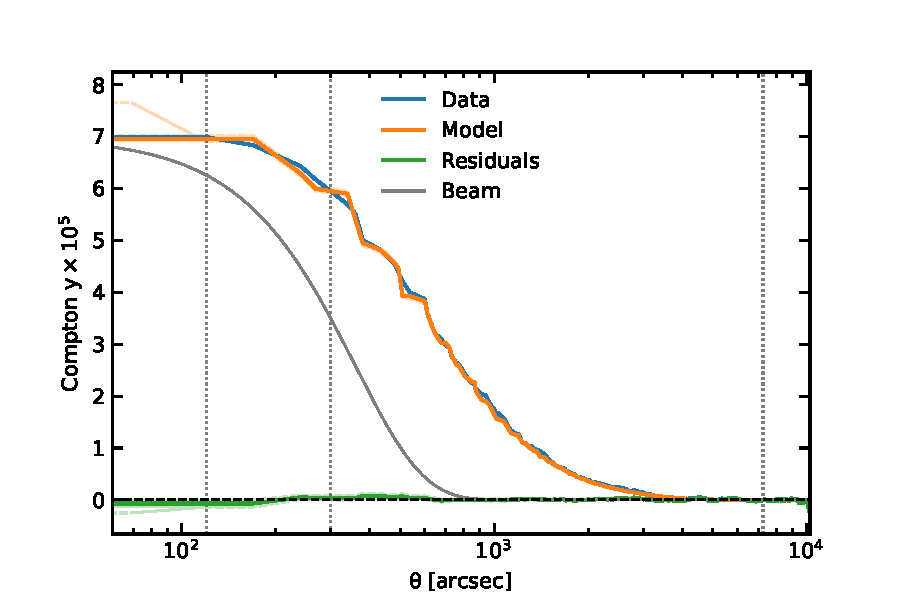
\includegraphics[height=4cm, trim={0 0 1cm 0.5cm}, clip]{../validation/results/C1/Planck/data_model_residuals_profiles.pdf}
    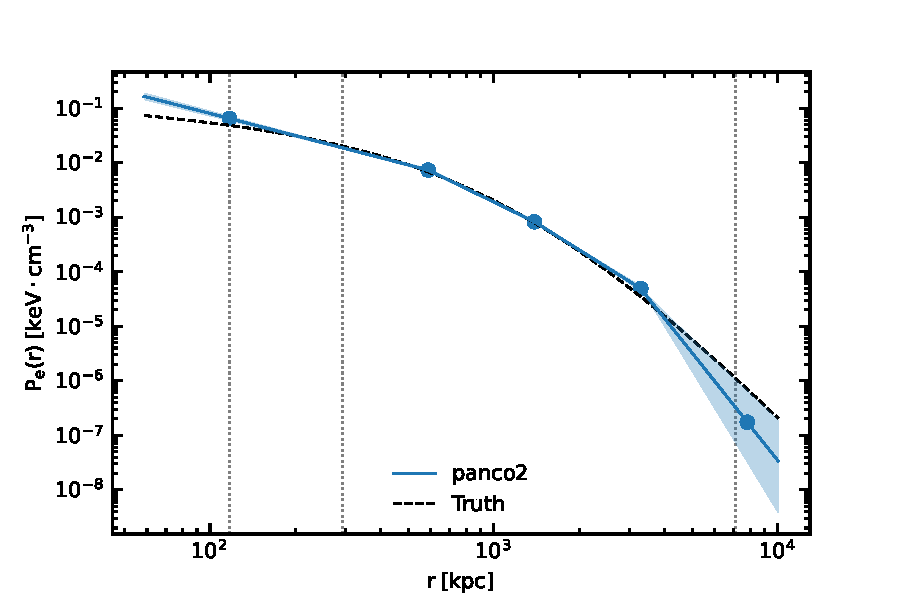
\includegraphics[height=4cm, trim={0 0 1cm 0.5cm}, clip]{../validation/results/C1/Planck/pressure_profile.pdf} \\
    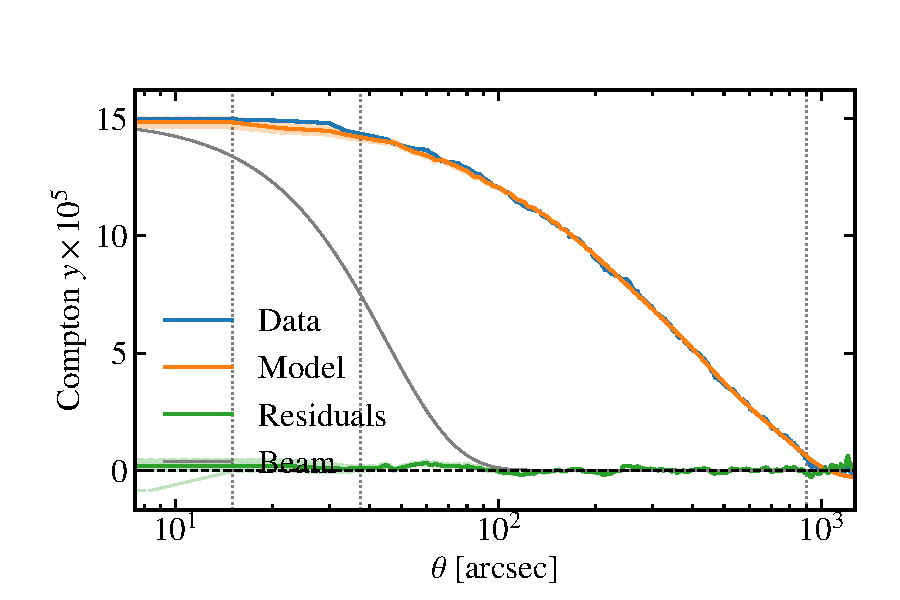
\includegraphics[height=4cm, trim={0 0 1cm 0.5cm}, clip]{../validation/results/C1/SPT/data_model_residuals_profiles.pdf}
    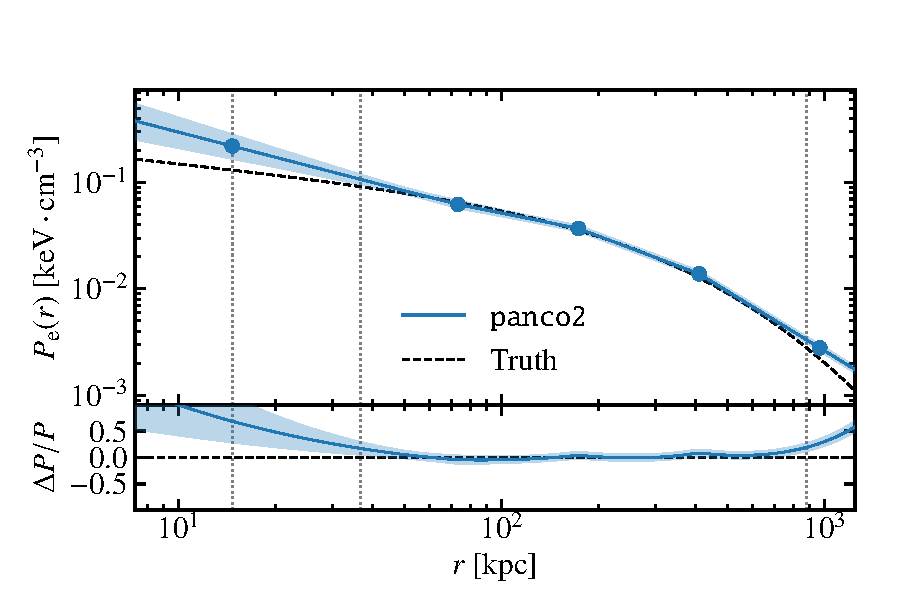
\includegraphics[height=4cm, trim={0 0 1cm 0.5cm}, clip]{../validation/results/C1/SPT/pressure_profile.pdf} \\
    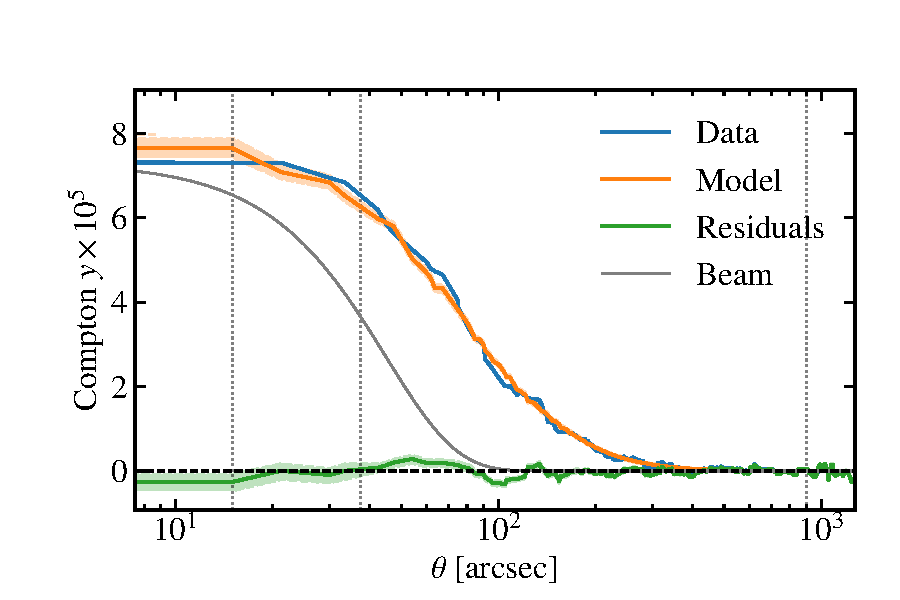
\includegraphics[height=4cm, trim={0 0 1cm 0.5cm}, clip]{../validation/results/C2/SPT/data_model_residuals_profiles.pdf}
    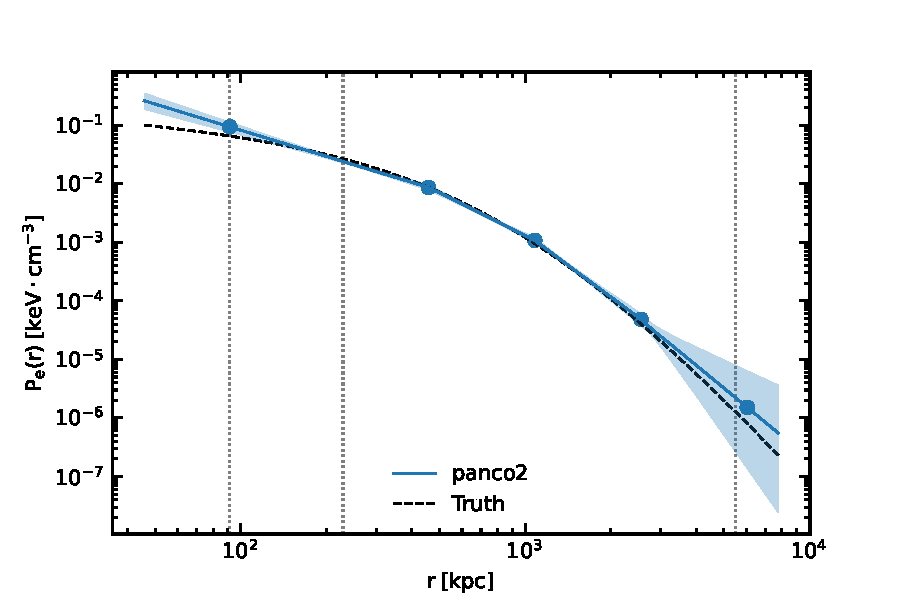
\includegraphics[height=4cm, trim={0 0 1cm 0.5cm}, clip]{../validation/results/C2/SPT/pressure_profile.pdf} \\
    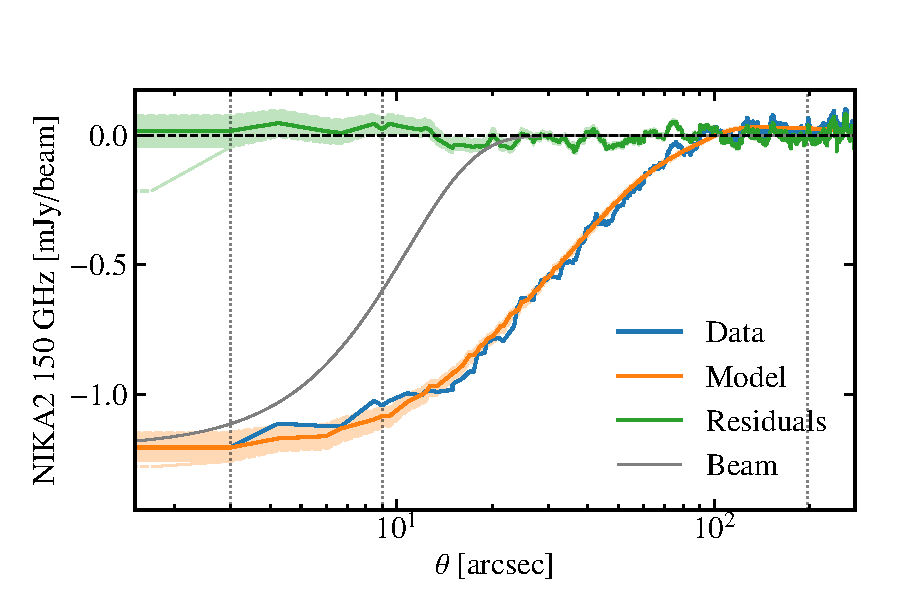
\includegraphics[height=4cm, trim={0 0 1cm 0.5cm}, clip]{../validation/results/C2/NIKA2/data_model_residuals_profiles.pdf}
    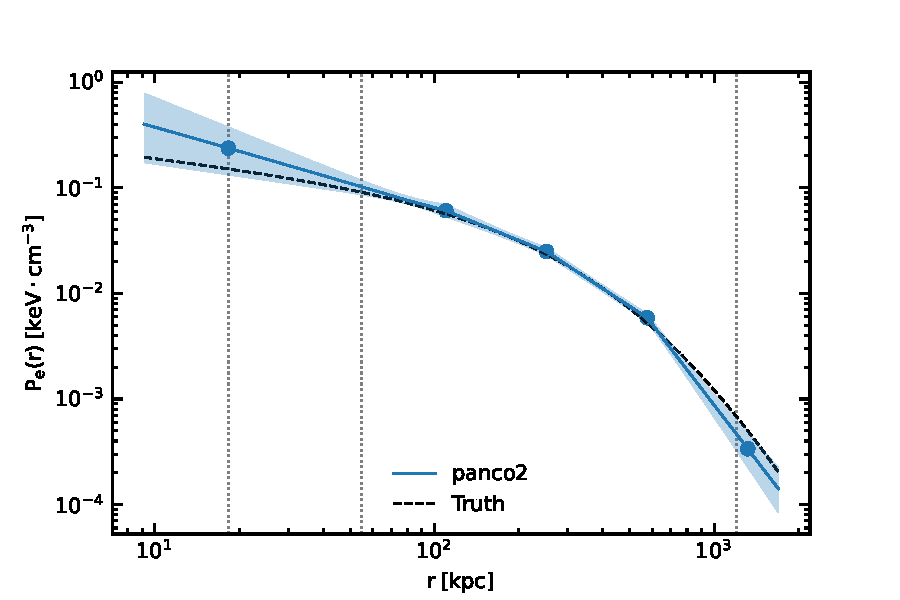
\includegraphics[height=4cm, trim={0 0 1cm 0.5cm}, clip]{../validation/results/C2/NIKA2/pressure_profile.pdf} \\
    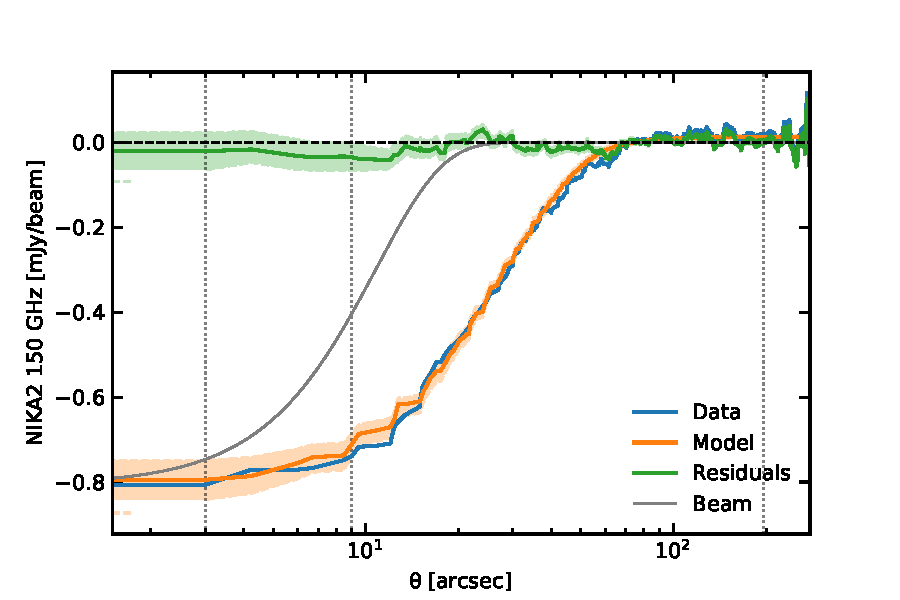
\includegraphics[height=4cm, trim={0 0 1cm 0.5cm}, clip]{../validation/results/C3/NIKA2/data_model_residuals_profiles.pdf}
    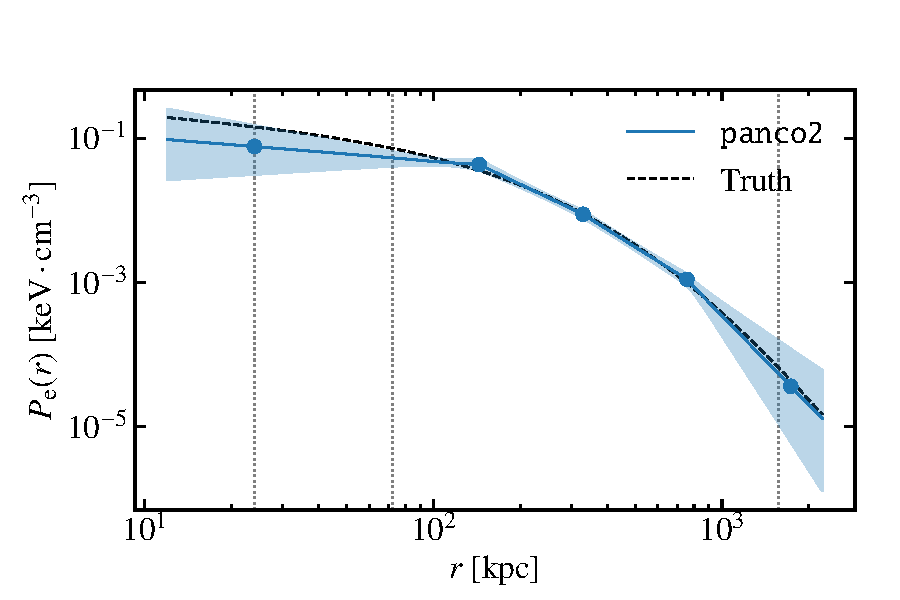
\includegraphics[height=4cm, trim={0 0 1cm 0.5cm}, clip]{../validation/results/C3/NIKA2/pressure_profile.pdf}
    \caption{
        \textbf{Left:} Data, model, and residuals (\ie\ difference between data and model) azimuthal profiles for the five validation fits.
        The beam profile is shown in grey for comparison.
        The rows are identical to Figure~\ref{fig:valid:dmr_2d}.
        For NIKA2 maps (bottom two rows), maps have been multiplied by $-1$ to show positive profiles.
        \textbf{Right:} Pressure profiles reconstructed for each validation fit (blue line).
        For each profile, the shaded area marks the region between the 16th and 84th percentiles of the posterior distribution.
        The dashed black line shows the true pressure profile used to generate each map.
        In each plot, dotted vertical lines, from left to right, show the size of a map pixel, the beam HWHM, and the half map size.
    }
    \label{fig:valid:profiles}
\end{figure*}
